\providecommand{\main}{../../..}
\documentclass[\main/dresen_thesis.tex]{subfiles}

\begin{document}
  \subsection{SuperADAM}\label{ch:lss:superadam}
    \begin{figure}[ht]
      \centering
      \includegraphics[width=0.7\textwidth]{appendix_instruments_superAdam}
      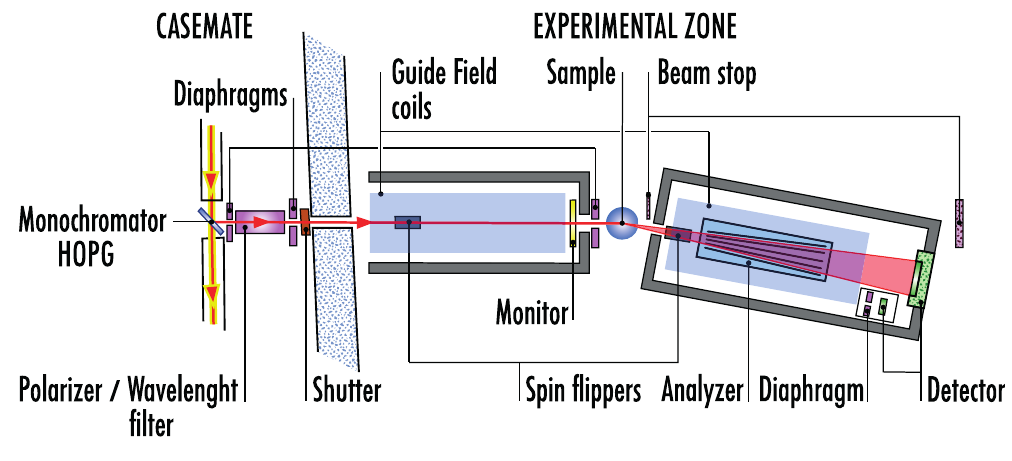
\includegraphics[width=0.7\textwidth]{appendix_instruments_superAdamSetup}
      \caption{\label{fig:lss:superadam}SuperADAM instrument at Institut Laue-Langevin, which is used for (polarized) neutron reflectometry (schematics reproduced from \cite{Devishvili_2015_Super}).}
    \end{figure}
    The SuperADAM instrument at the Institut Laue-Langevin is a polarized neutron reflectometer, which can be used to study thin-layer samples in the order of up to $300 \unit{nm}$.
    The instrument is an upgrade of the earlier reflectometer ADAM (Advanced Diffractometer for the Analysis of Materials) and is operated by VR, The Swedish Research Council.
    It is part of the Collaborative Research Group (CRG) system at ILL.

    The optimal wavelength for a high neutron flux is set at $5.183 \unit{\angstrom}$.
    The incident polarization is in the order of $97 - 99 \unit{\%}$ and the wavelength spread relatively low with $0.5 \unit{\%}$ (standard deviation) and therefore the instrumental resolution is mainly determined by the collimation.
    The $^3\mathrm{He}$ detector has $1400 \times 1400$ pixels with a quadratic size of $0.214 \unit{mm}$ per pixel and a resolution of $2.8 \unit{mm}$ (FWHM).
    Using a cryostat, samples can be cooled down to $2 \unit{K}$ and by means of an electromagnet a magnetic field of up to $1.1 \unit{T}$ can be applied.

\end{document}